% Figure 1 — Three-domain conceptual model of the SSCI (Section 3.1).
% Standalone TikZ; compiles to a cropped PDF with pdflatex, and can also be
% \input into main.tex inside a figure environment.
\documentclass[border=4pt]{standalone}
\usepackage{tikz}
\usepackage{amsmath}
\usepackage{xcolor}
\definecolor{okorange}{RGB}{230,159,0}
\definecolor{oksky}{RGB}{86,180,233}
\definecolor{okblue}{RGB}{0,114,178}
\usetikzlibrary{positioning,arrows.meta,backgrounds,fit}
\begin{document}
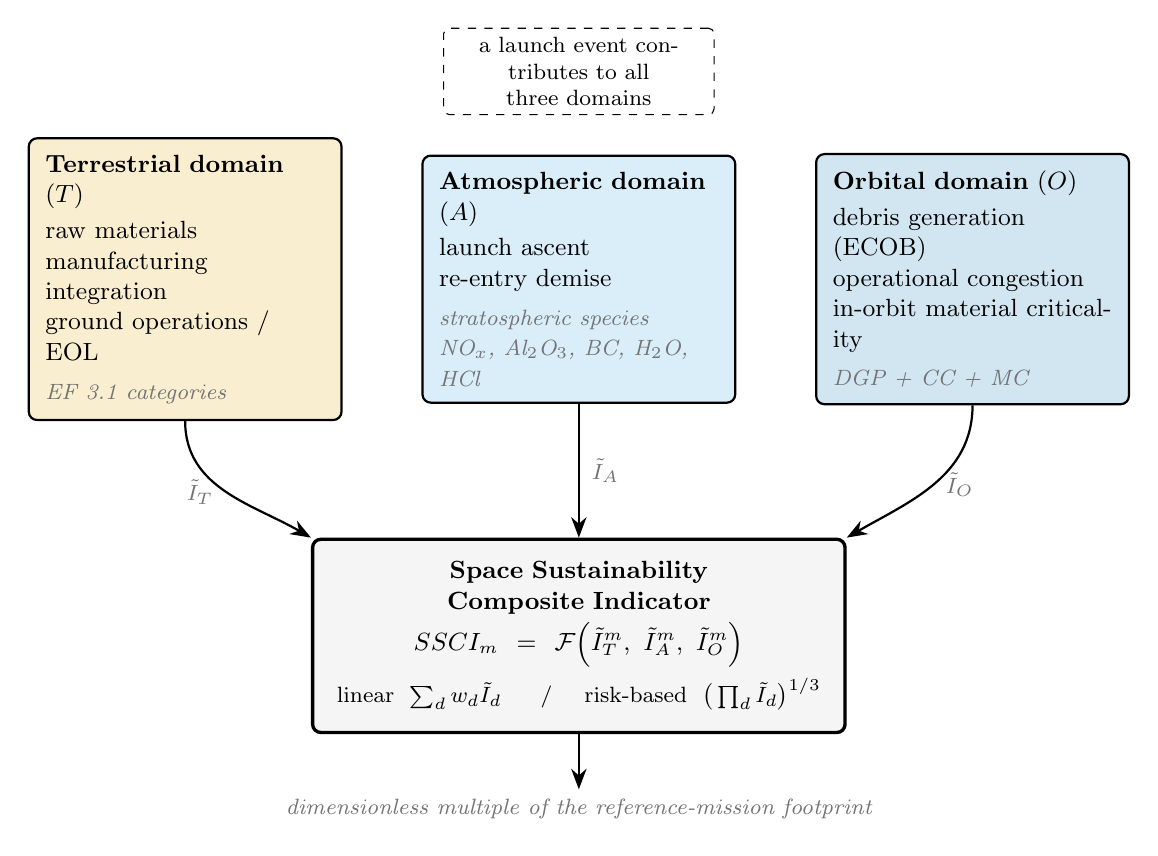
\begin{tikzpicture}[
  font=\small,
  dombox/.style={rounded corners=3pt, draw, thick, align=left,
                 inner sep=6pt, text width=3.55cm, minimum height=2.9cm},
  alab/.style={font=\footnotesize\itshape, text=black!55},
  ssci/.style={rounded corners=3pt, draw, very thick, align=center,
               inner sep=8pt, text width=6.2cm, fill=black!4},
  flow/.style={-{Stealth[length=2.6mm]}, thick},
]

% --- three domain boxes ---
\node[dombox, fill=okorange!18] (T) {%
  \textbf{Terrestrial domain} ($T$)\\[2pt]
  raw materials\\ manufacturing\\ integration\\ ground operations / EOL\\[3pt]
  {\footnotesize\itshape\color{black!55} EF 3.1 categories}};
\node[dombox, fill=oksky!22, right=1.0cm of T] (A) {%
  \textbf{Atmospheric domain} ($A$)\\[2pt]
  launch ascent\\ re-entry demise\\[3pt]
  {\footnotesize\itshape\color{black!55} stratospheric species}\\
  {\footnotesize\itshape\color{black!55} NO$_x$, Al$_2$O$_3$, BC, H$_2$O, HCl}};
\node[dombox, fill=okblue!18, right=1.0cm of A] (O) {%
  \textbf{Orbital domain} ($O$)\\[2pt]
  debris generation (ECOB)\\ operational congestion\\ in-orbit material criticality\\[3pt]
  {\footnotesize\itshape\color{black!55} DGP + CC + MC}};

% --- composite node ---
\node[ssci, below=1.7cm of A] (S) {%
  \textbf{Space Sustainability Composite Indicator}\\[2pt]
  $SSCI_m=\mathcal{F}\!\left(\tilde{I}_T^m,\ \tilde{I}_A^m,\ \tilde{I}_O^m\right)$\\[3pt]
  {\footnotesize linear $\;\sum_d w_d\tilde I_d\;$ \quad / \quad risk-based $\;\big(\textstyle\prod_d \tilde I_d\big)^{1/3}$}};

\draw[flow] (T.south) to[out=-90,in=150]
  node[midway, left=1pt, alab] {$\tilde I_T$} (S.north west);
\draw[flow] (A.south) -- node[midway, right=1pt, alab] {$\tilde I_A$} (S.north);
\draw[flow] (O.south) to[out=-90,in=30]
  node[midway, right=1pt, alab] {$\tilde I_O$} (S.north east);

% --- output ---
\node[below=0.7cm of S, font=\footnotesize\itshape, text=black!55]
  (out) {dimensionless multiple of the reference-mission footprint};
\draw[flow] (S.south) -- (out.north);

% --- shared-process note ---
\node[draw, dashed, rounded corners=2pt, font=\footnotesize, align=center,
      text width=3.2cm, above=0.5cm of A]
  {a launch event contributes to all three domains};
\end{tikzpicture}
\end{document}
